\documentclass[cn]{elegantbook}

\usepackage{tikz}
\usepackage{graphicx}
\usepackage{subcaption}
\usepackage[ruled,linesnumbered,vlined]{algorithm2e}
\usepackage{hyperref}
\usepackage{listings}
\usepackage{interval}

\intervalconfig{
  soft open fences,
}

\def\figureautorefname{图}

\SetAlgorithmName{算法}{算法}{算法索引}

\renewcommand*{\lstlistingname}{代码}

\title{何老师算法课笔记}
\subtitle{还没有想好的副标题}
\author{计卓1801全体}
\institute{华中科技大学}
\date{\zhtoday}
\version{1.2.0}
\logo{logo.png}
\cover{cover.png}

\begin{document}
\maketitle
\tableofcontents
\pagenumbering{arabic}

% add your code here
\chapter{Example}

\begin{introduction}
\item 提要1
\item 提要2
\item 提要3
\item 提要4
\item 提要5
\end{introduction}

这是一个示例。

\section{环境}

\begin{theorem}{xxx定理}{label-for-this-theorem}
  这是一个定理。
\end{theorem}

\begin{example}
  这是一个例题。
\end{example}

\begin{definition}{xxx}{label-for-this-def}
  这是一个定义。
\end{definition}

\begin{lemma}{xxx引理}{label-for-this-lemma}
  这是一个引理。
\end{lemma}

\begin{proposition}{xxx命题}{label-for-this-prop}
  这是一个命题。
\end{proposition}

这是一个列表:

\begin{itemize}
  \item first thing
  \item second thing
    \begin{itemize}
      \item more of second thing
    \end{itemize}
  \item third thing
    \begin{enumerate}
      \item 可以是有序列表
      \item more of enumerate
    \end{enumerate}
\end{itemize}

这是一张图片:

\begin{figure}[hbt]
  \centering
  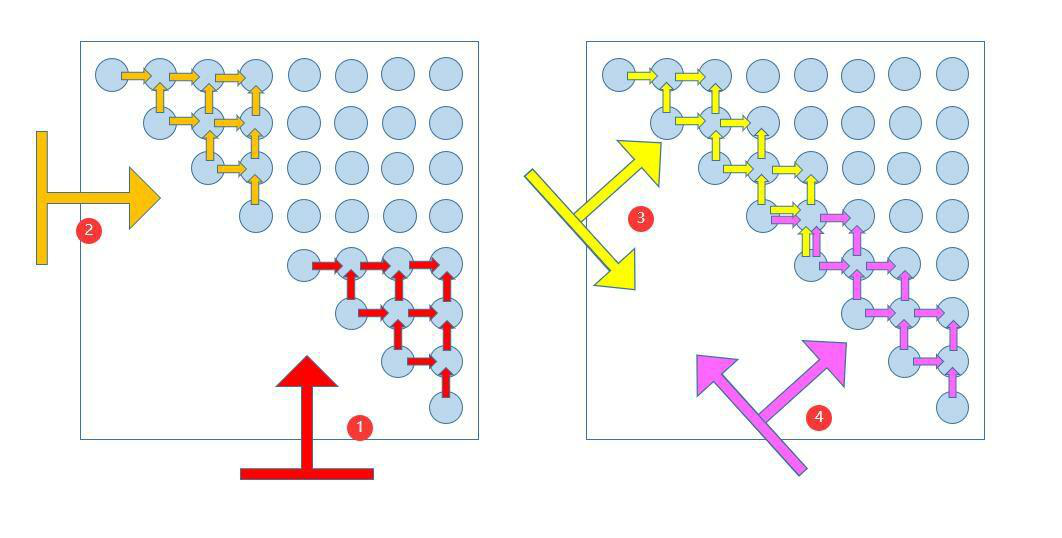
\includegraphics{image/dynamic-programming-1.png}
  \caption{这是一张图片}\label{fig:example}
\end{figure}

这是一段代码:

\begin{lstlisting}[language=Python, caption=Python example]
import numpy as np

def incmatrix(genl1,genl2):
    m = len(genl1)
    n = len(genl2)
    M = None #to become the incidence matrix
    VT = np.zeros((n*m,1), int)  #dummy variable

    #compute the bitwise xor matrix
    M1 = bitxormatrix(genl1)
    M2 = np.triu(bitxormatrix(genl2),1)

    for i in range(m-1):
        for j in range(i+1, m):
            [r,c] = np.where(M2 == M1[i,j])
            for k in range(len(r)):
                VT[(i)*n + r[k]] = 1;
                VT[(i)*n + c[k]] = 1;
                VT[(j)*n + r[k]] = 1;
                VT[(j)*n + c[k]] = 1;

                if M is None:
                    M = np.copy(VT)
                else:
                    M = np.concatenate((M, VT), 1)

                VT = np.zeros((n*m,1), int)

    return M
\end{lstlisting}

更多环境请见文档。

\section{引用}

\subsection{交叉引用}

引用定理~\ref{thm:label-for-this-theorem}。

\subsection{参考文献}

引用一个参考文献~\cite{cormen2009introduction}

\chapter{动态规划(1)}

\begin{introduction}
  \item 带权区间调度
  \item 矩阵链乘法
\end{introduction}

\section{概述}
在前面的课程中,已经学习过了贪心法和分治法两种策略,本章将开始动态规划(Dynamic programming)的学习。
简要比较一下几种算法策略的不同。

\begin{itemize}
  \item 贪心法 -基于贪心策略,每次总是选取眼前最优的选项,同时期待最终的结果最优。
        优点在于思考和模型建立较为简单,难点在于如何证明算法的正确性。
  \item 分治法 -分而治之,子问题不存在重叠。
        难点在于如何分割问题,以及如何合并解。
  \item 动态规划 -思想类似于分治,与贪心法相反,子问题之间存在重叠,算法执行过程中记录子问题的解。
        难点在于如何找到转移方程。
\end{itemize}

本章将介绍动态规划在带权区间调度~\ref{sec:weighted-interval-scheduling} 、矩阵链乘法~\ref{sec:matrix-chain-multiplication} 两个问题上的应用。

\section{带权区间调度}\label{sec:weighted-interval-scheduling}

\subsection{问题描述}

\begin{figure}[hbt!]
  \centering
  \begin{tikzpicture}
    \draw[|-|] (0, 5) -- node [above] {$w_1=2$} (2, 5);
    \draw[|-|] (1, 4) -- node [above] {$w_2=4$} (5, 4);
    \draw[|-|] (3, 3) -- node [above] {$w_3=4$} (7, 3);
    \draw[|-|] (1.5, 2) -- node [above] {$w_4=7$} (8.5, 2);
    \draw[|-|] (8, 1) -- node [above] {$w_5=2$} (10, 1);
    \draw[|-|] (9.5, 0) -- node [above] {$w_6=1$} (10.5, 0);
  \end{tikzpicture}
  \caption{区间调度示例}\label{fig:wis-picture-1}
\end{figure}

下面给出带权区间调度问题的定义。

\begin{definition}{带权区间调度问题}{def:weighted-interval-scheduling}
  给定区间$I_1, I_2, \ldots, I_n$,
  $s_i$为$I_i$开始时间,$f_i$为$I_i$的结束时间($f_i>s_i$),$w_i>0$, 假设$\forall i < j$,$ s_i<s_j$。
  \begin{itemize}
    \item $OPT(k)$:表示区间集合$\{ I_1, I_2, \ldots , I_i \}$上的最优解权值。
    \item $P(i)$:表示$I_i$的前驱,当$P(i)=j$时,有$f_j=\max\limits_{1 \leq k < i}\{f_k | f_k < s_i\}$,当$I_i$没有前驱时,$P(i)=0$
  \end{itemize}
  目标:寻找一个$\sum w_i$最大的区间子集$R$,满足$\forall I_m,I_n \in R, m < n \text{都有} f_m < s_n$。
\end{definition}

通俗来讲,就是找出一个彼此时间不重叠的区间序列,使得这个序列的权重在所有可能的序列中,权重最大。

\begin{remark}
  以\autoref{fig:wis-picture-1}为例,$P(6)=4, P(5)=3, P(4)=0, P(3)=1, P(2)=0, P(1)=0$
\end{remark}

\subsection{贪心}

\begin{figure}[hbt!]
  \centering
  \begin{subfigure}{.3\textwidth}
    \centering
    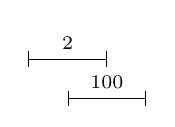
\begin{tikzpicture}
      \draw[|-|] (0, 0) -- node [above] {\scriptsize 2} (1, 0);
      \draw[|-|] (0.5 , -0.5) -- node [above] {\scriptsize 100} (1.5, -0.5);
    \end{tikzpicture}
    \caption{}\label{fig:wis-counterexample1}
  \end{subfigure}
  \begin{subfigure}{.3\textwidth}
    \centering
    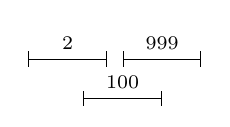
\begin{tikzpicture}
      \draw[|-|] (0, 0) -- node [above] {\scriptsize 2} (1, 0);
      \draw[|-|] (1.2, 0) -- node [above] {\scriptsize 999} (2.2, 0);
      \draw[|-|] (0.7 , -0.5) -- node [above] {\scriptsize 100} (1.7, -0.5);
    \end{tikzpicture}
    \caption{}\label{fig:wis-counterexample2}
  \end{subfigure}
  \begin{subfigure}{.3\textwidth}
    \centering
    \begin{tikzpicture}
      \draw[|-|] (0, 0) -- node [above] {\scriptsize 2} (1, 0);
      \draw[|-|] (1.2, 0) -- node [above] {\scriptsize 3} (2.2, 0);
      \draw[|-|] (0.7 , -0.5) -- node [above] {\scriptsize 6} (1.7, -0.5);
    \end{tikzpicture}
    \caption{}\label{fig:wis-counterexample3}
  \end{subfigure}
  \caption{贪心反例}\label{fig:wis-counterexample}
\end{figure}

\begin{enumerate}
  \item 以最早完成时间排序,反例如\autoref{fig:wis-counterexample1}
  \item 以最大权重排序,反例如\autoref{fig:wis-counterexample2}
  \item 选择冲突最少的区间,反例如\autoref{fig:wis-counterexample3}
\end{enumerate}

常见的贪心思考方向无法解决带权区间调度问题。

\subsection{动态规划}

\subsubsection{算法设计}
观察带权区间调度问题,对于最优解$OPT(n)$,可以得到如下两个结论:
\begin{itemize}
  \item 子集$R$要么包含$I_n$,要么不包含$I_n$
  \item 对于区间$I_n$
        \begin{itemize}
          \item 如果$I_n \in R$,$OPT(n)=w_n+OPT(P(n))$
          \item 如果$I_n \notin R$,$OPT(n)=OPT(n-1)$
        \end{itemize}
\end{itemize}

于是我们可以得到该问题的状态转移方程:
\begin{equation}
  OPT(n) = \begin{cases}
    w_n + OPT(P(n)), & I_n \in R    \\
    OPT(n-1),        & I_n \notin R
  \end{cases}
\end{equation}
\par
因为需要找到最大的权值,上式也可以写成
\begin{equation}
  OPT(n)=\max \{w_n+OPT(P(n)),OPT(n-1)\}
\end{equation}

\subsubsection{算法分析}

\paragraph*{时间复杂度}
在记录最优解的情况下,仅需要填满大小为$n$的一维数组即可,每次计算$OPT(n)$时会从数组中取已计算的$OPT(n-1)$,因此时间复杂度为$O(n)$。
考虑不记录子问题解的情况,在最坏情况下$T(n)=T(n-1)+T(n-2)$,可以发现这是一个斐波那契序列,因此求解该问题的时间复杂度约为$O(1.618^n)$。
\paragraph*{空间复杂度}
算法执行过程中,会开辟一个空间记录子问题最优解,即空间复杂度为$O(n)$。

\section{矩阵链乘法}\label{sec:matrix-chain-multiplication}

\subsection{问题描述}
假设有矩阵乘法$A \cdot B \cdot C$。其中$A = (n \times m), B = (m \times n), C = (n \times m)$。
根据矩阵乘法性质,有$(A \cdot B) \cdot C = A \cdot (B \cdot C)$。
前者的时间复杂度为$O(2n^2m)$,后者的时间复杂度为$O(2m^2n)$。
于是我们可以看出,不同的矩阵相乘顺序,对结果没有影响,但是对计算时间却有较大的影响,矩阵链乘法即是找到一个最优的相乘顺序。
\par
下面给出矩阵链乘法问题的相关定义。
\begin{definition}{矩阵链乘法问题}{def:matrix-chain-multiplication}
  给定n个矩阵的链$<A_1,A_2,\ldots,A_n>$矩阵$A_i$的规模为$p_{i-1} \times p_i, (1 \leq i \leq n)$。
  求完全括号化方案,使得计算矩阵乘积$A_1 \cdot A_2 \cdot A_3 \cdots A_n$所需的标量乘法次数最少。
  \begin{itemize}
    \item $C(i,j,k)$:记$\underbrace{(A_i \cdot A_{i+1} \cdots A_j)}_{p \times q}  \cdot \underbrace{(A_{j+1} \cdot A_{j+2} \cdots A_k)}_{q \times r}$相乘的代价为$C(i,j,k)=pqr$。
    \item $OPT(i,j)$:记矩阵链$<A_i \cdots A_j>$之间的最优相乘成本为$OPT(i,j)$。
  \end{itemize}
\end{definition}

\subsection{算法设计}
对于矩阵链$<A_i \cdots A_j>$,我们可以在$i$到$j$之间找到一个切分点$k$,将问题分解为$<A_i \cdots A_k>$和$<A_{k+1} \cdots A_j>$两个子问题。
假设这两个子问题的最优解已知(在动态规划中,可以理解为已存在子问题解的记录),那么可以得到如下的公式。
\begin{equation}
  OPT(i,j) = \begin{cases}
    0,                                                            & i = j \\
    \min\limits_{i \leq k < j} \{ OPT(i,k)+OPT(k+1,j)+C(i,k,j)\}, & i < j
  \end{cases}
\end{equation}

\begin{remark}
  根据算法执行的迭代方向不同,公式可以有多种写法,几种迭代方向参见\autoref{fig:mcm-fig1}
\end{remark}

\begin{algorithm}
  \caption{MATRIX-CHAIN-ORDER}\label{alg:mco}
  \KwIn{序列$p=<p_0,p_1,\ldots,p_n>$,长度为$n+1$,$p_{i-1} \times p_i$为第$i$个矩阵的规模}
  \KwOut{代价表$OPT[1..n, 1..n]$,分割表$s[1..n-1, 2..n]$记录$OPT(i,j)$的分割点$k$}
  \BlankLine{}
  $n = p.length-1$\;
  $\text{let } OPT[1..n, 1..n] \text{ and } s[1..n-1, 2..n] \text{ be new tables}$\;
  \For{$i = 1$ \KwTo$n$}{$OPT[i,i]=0$\;}
  \For{$l = 2$ \KwTo$n$}{
  \For{$i = 1$ \KwTo$n-l+1$}{
  $j = i+l-1$\;
  $OPT[i,j] = \infty$\;
  \For{$k = i$ \KwTo$j-1$}{
  $q = OPT[i,k]+OPT[k+1,j]+p_{i-1} p_k p_j$\;
  \If{$q < OPT[i,j]$}{
    $OPT[i,j] = q$\;
    $s[i,j] = k$\;
  }
  }
  }
  }
  \Return{OPT and s}
\end{algorithm}

\begin{figure}[hbt!]
  \centering
  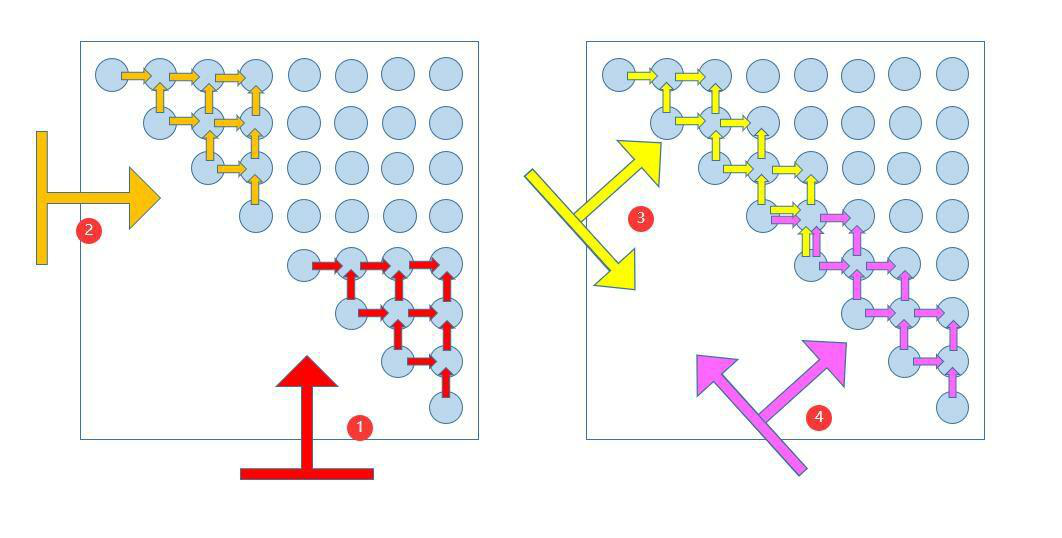
\includegraphics[scale=0.6]{image/dynamic-programming-1.png}
  \caption{几种不同的迭代方向}\label{fig:mcm-fig1}
\end{figure}

\subsection{算法分析}
\paragraph*{时间复杂度}
简单分析\autoref{alg:mco}的嵌套循环结构,可以得到算法的运行时间为$O(n^3)$。
循环嵌套的深度为三层,每层的循环变量$(i\text{、}j\text{和}k)$最多取$n-1$个值。
\paragraph*{空间复杂度}
需要$O(n^2)$的空间来保存$OPT$和$s$。

\chapter{网络流应用}

\begin{introduction}
\item 最大二分匹配问题
\item Tiling Problem
\item 棒球比赛
\item 项目选择
\end{introduction}

本章是在基于网络流FF算法的基础上,学习网络流的应用。

\section{最大二分匹配问题}

\begin{definition}{二分图}{def1}
    对于无向图\(G = (V,\,E)\),若顶点集V可以分割为两个互不相交子集\((X,\,Y)\),使得边集\(E\)中任意一条边\(e = (u,\,v)\),都可以满足\(u \in X\) ,\(v \in Y\),则称图\(G\)为二分图。
\end{definition}

问题: 对于给定的\(G = (V,\,E)\),\(V\)为\(V_l \cup V_r\),\(V_l \cap V_r = \phi\),找到\(V_l\)到\(V_r\)的最大匹配。

\begin{definition}{匹配}{def2}
    一边集M为边集E的子集,且M中任意两条边无公用顶点(不相交),则称M为图G的一个匹配。
\end{definition}

\begin{definition}{极大匹配}{def3}
    不是其他任何匹配的子集的匹配。
\end{definition}

\begin{definition}{最大匹配}{def4}
    极大匹配中包含最多边数的一个匹配称为最大匹配。
\end{definition}

\begin{figure}[htb]
  \centering
  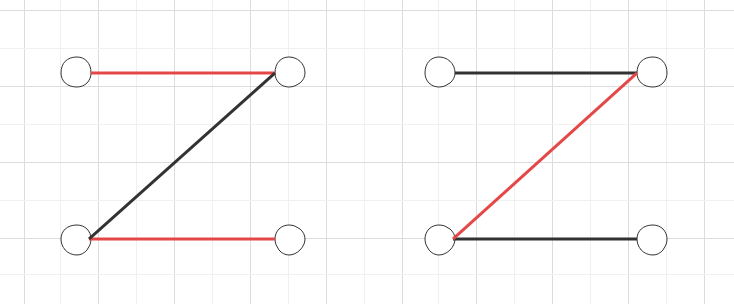
\includegraphics[scale=0.6]{image/networkflow1.png}
  \caption{极大匹配举例}\label{fig1}
\end{figure}
如\autoref{fig1}所示,二者都为极大匹配,但是只有左图为最大匹配。

\begin{figure}[htb]
  \centering
  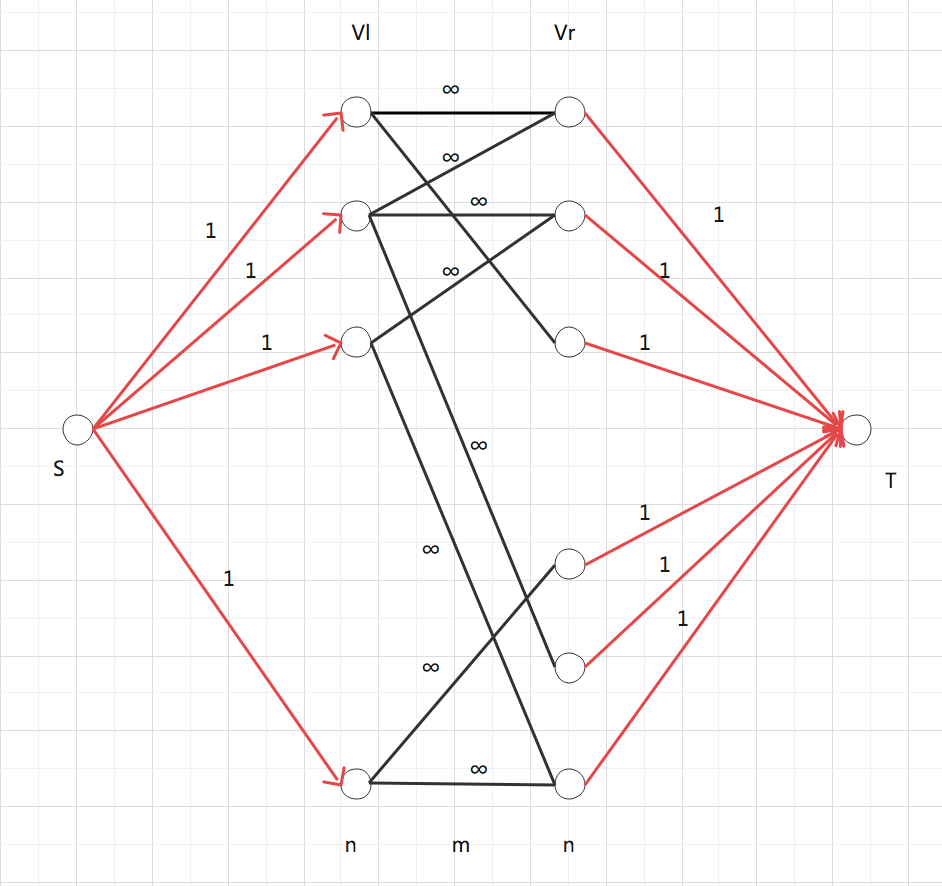
\includegraphics[scale=0.6]{image/networkflow2.png}
  \caption{FF算法建模}\label{fig2}
\end{figure}

使用如\autoref{fig2}的方法构建网络流,之后使用FF算法求解。

网络流解决最大二分匹配问题的时间复杂度为:\(O(mn)\)。

\begin{lemma}{最大流最小割定理}{lemma1}
    指在一个网络流中,能够从源点到达汇点的最大流量等于如果从网络中移除就能够导致网络流中断的边的集合(对割的另一种理解)的最小容量和。即在任何网络中,最大流的值等于最小割的容量。
\end{lemma}

使用下面一个例子说明该算法的正确性:
\begin{figure}[htb]
  \centering
  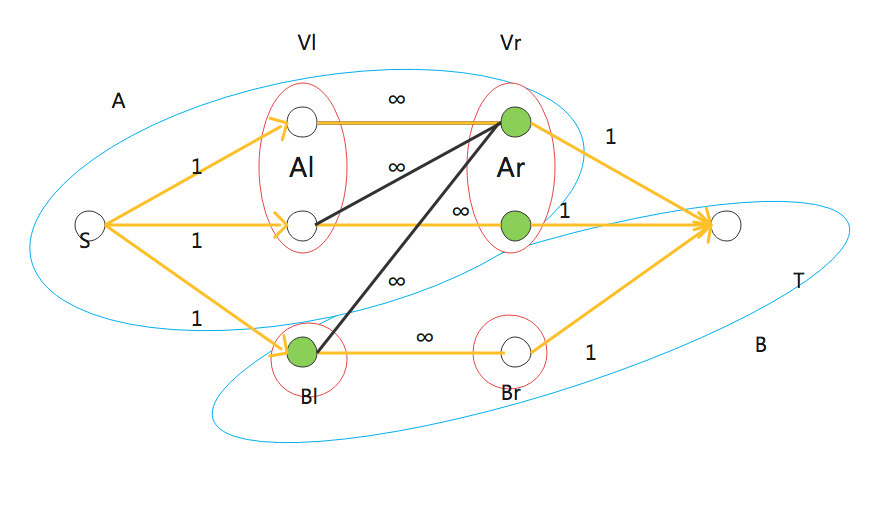
\includegraphics[scale=0.6]{image/networkflow3.png}
  \caption{算法正确性说明}\label{fig3}
\end{figure}

\begin{example}
  如\autoref{fig3}所示,给定二分图中,点被分为了\(V_l\)和\(V_r\)两个部分,构造网络流算法,设置一个起点S,且令S到所有的Vl中的点均有路径,容量为1;设置一个终点T,且从\(V_r\)中的点到T均有路径,容量为1。同时,所有\(V_l\)与\(V_r\)之间的路径容量均设为无穷大,由此可以找到该网络流的最大流和最小割。
\end{example}

\begin{itemize}
  \item 因为最大流等价于最小割,对于残差图Gf,从S点可以到达的点构成集合A,其他点构成集合B。
  \item 因为该图为二分图,所以不存在从\(A_l\)到\(B_l\)的路径,同样的,也不存在从\(A_r\)到\(B_r\)的路径。
  \item 因为找到了最小割,而且最小割是有限数,因此不存在从\(A_l\)到\(B_r\)的路径(已知\(A_l\)到\(B_r\)的边的容量为正无穷)。
  \item 最小割值 \(C(A,B) = |B_l|\)(实际为S流入\(B_l\)) + |\(A_r\)|(实际为\(A_r\)流入T) = 最大流 = 最大匹配。
\end{itemize}
对于二分图来说 |最大匹配|=|最小顶点覆盖|。

\begin{definition}{完美匹配}{def5}
    所有的点均被匹配,不存在未被匹配的点。
\end{definition}

\begin{definition}{T(A)}{def6}
  \(A \subseteq V_l\),\(T(A) = \{b \in Vr | (a,b) \in E \}\)。
\end{definition}

对于一个二分图来说,如果\(|V_l|=|V_r|=n\),并且存在完美匹配,那么任取集合\(A \subseteq V_l,\,|T(A)| \ge |A|\)。

\begin{theorem}{霍尔定理}{thm1}
  任取\(A \subseteq V_l\),若\(|T(A)| \ge |A|\),则存在完美匹配。
\end{theorem}
证明霍尔定理的正确性(证明其逆否命题正确):
\begin{itemize}
  \item 逆否命题:若不存在完美匹配,则存在集合A,\(|T(A)| < |A|\)。
  \item \(|V_l|=|V_r|=n\),所以最大匹配\(k<n\)。
  \item 找到A,B(即S-T割),\(C(A,B) = f(A,B) = k<n\)。
  \item \(|A_l|+|B_l| = n,\,|B_l|+|A_r| = k < n\)。由此可以推出\(|A_l| > |A_r|\),可以推出\(|T(A_l)| < |A|\)。
  \item 因此,逆否命题成立,霍尔定理得证。
\end{itemize}

\section{骨牌问题}
回顾本课程开头提到的骨牌问题,我们试着用网络流的方法再次解决。
\begin{example}
    在\(m \times n\)的残缺棋盘(有方格缺失)上,填入\(1 \times 2\)大小的矩形骨牌,能否用骨牌将棋盘填满?
\end{example}

\begin{figure}[htb]
  \centering
  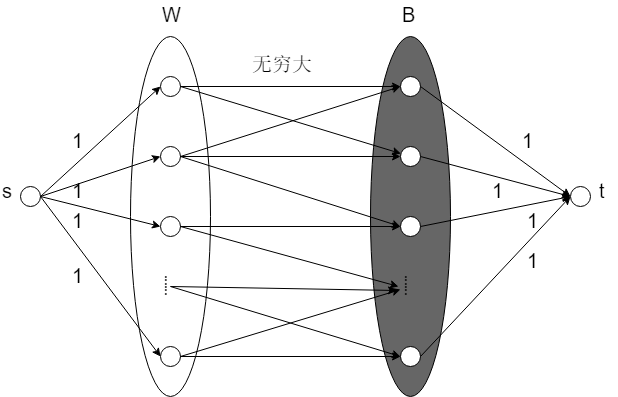
\includegraphics[scale=0.6]{image/networkflow4.png}
  \caption{骨牌问题建模}\label{fig4}
\end{figure}

\begin{itemize}
    \item 问题建模:沿用之前的处理方法,黑白相间地将棋盘做上标记,
        这样棋盘的方格会被分为两个集合\((B,W)\)。
        若\(|B|\)不等于\(|W|\),我们可以得出否定的结论;
        若\(|B|=|W|=n\),则在B和W集之间,相邻的方格连上边,容量正无穷,
        这样一来,(B,W) 相当于二分匹配中的\((V_l,\,V_r)\),
        就相当于解决一个最大二分匹配问题,建模如\autoref{fig4}。
\end{itemize}

求得最大流\(f=n\),则表示该棋盘可以用骨牌填满。
\begin{itemize}
 \item 算法复杂度分析:F-F算法复杂度为\(O(mC)\),在这个模型中,m=n,\(C \le 4n\),所以用网络流解决棋盘问题的算法时间复杂度为\(O(n^2)\)。
\end{itemize}

\section{棒球比赛}
\begin{figure}[htb]
  \centering
  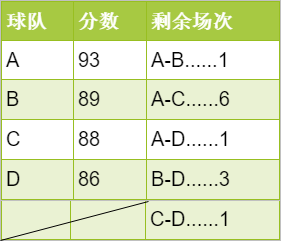
\includegraphics[scale=0.6]{image/networkflow5.png}
  \caption{棒球问题说明}\label{fig5}
\end{figure}
\begin{example}
有四个棒球队比赛,目前赛场上的得分情况及剩余的场次如\autoref{fig5},问B队有没有机会赢得比赛(并列第一也算赢)?
\end{example}

\begin{figure}[h]
  \centering
  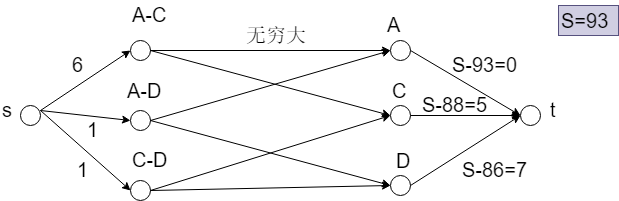
\includegraphics[scale=0.6]{image/networkflow6.png}
  \caption{棒球问题建模}\label{fig6}
\end{figure}

\begin{itemize}
  \item 问题建模:先计算若B队赢得了剩下所有可赢得的分后的总得分S。称参赛双方相同的比赛为一类比赛。将每类比赛作为顶点,通过容量为该类比赛剩余场数的入边交于源点s,出边指向参赛队伍,容量为正无穷;参赛队伍出边指向汇点t,容量为S-(该队伍的当前得分)。如\autoref{fig6}所示。
\end{itemize}

求得最大流\(f = C_{in}(t)\) ,\(C_{in}(t)\)即t的流入边容量之和,则表示B有机会赢。

\begin{figure}[htb]
  \centering
  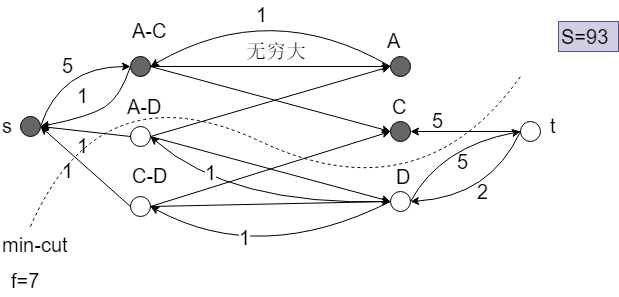
\includegraphics[scale=0.6]{image/networkflow7.png}
  \caption{棒球问题残差图}\label{fig7}
\end{figure}

\begin{itemize}
  \item 用F-F算法求模型的最大流和最小割,残差图如\autoref{fig7}。
\end{itemize}
\begin{example}
如果初始状态,B的得分为90,那么B能否获胜?(B有机会获胜)
\end{example}

\section{项目选择问题}
\begin{example}
有一项目的集合\{1,2,……,n\},项目之间有一定相互制约关系,完成每个项目都有一个价值\(v_i\),\(v_i\)可正可负。现要求一子集A,使得总价值p最大,且A中任一项目的前驱任务(完成一项目之前所必须完成的项目)也必须在A中。
\end{example}

\begin{figure}[htb]
  \centering
  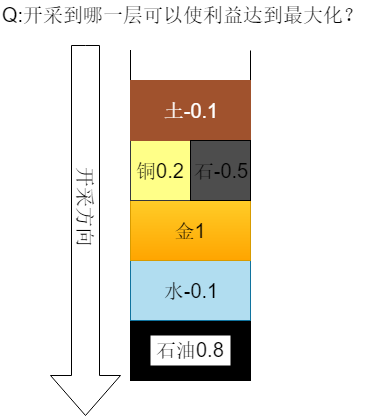
\includegraphics[scale=0.6]{image/networkflow8.png}
  \caption{项目选择事例}\label{fig8}
\end{figure}
为更好地理解问题,给出一更加具体地例子,如\autoref{fig8}所示。
\begin{figure}[htb]
  \centering
  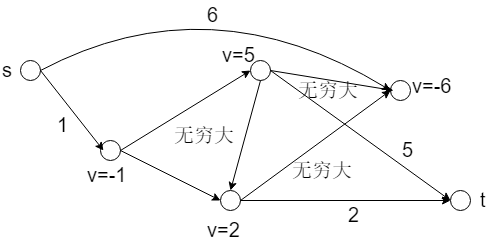
\includegraphics[scale=0.6]{image/networkflow9.png}
  \caption{项目选择建模}\label{fig9}
\end{figure}
\begin{itemize}
  \item 问题建模:由于有先后的制约关系,所以原图应为一个有向图,在此基础上,引入源点s,指向所有价值为负的项目,容量为该项目价值的绝对值;所有价值为正的项目指向汇点t,容量为该项目的价值。对一实例的建模如\autoref{fig9}。
\end{itemize}

\begin{figure}[htb]
  \centering
  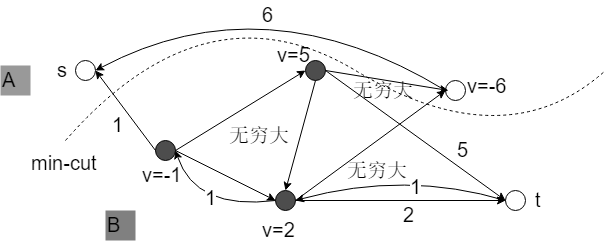
\includegraphics[scale=0.6]{image/networkflow10.png}
  \caption{项目选择问题解决}\label{fig10}
\end{figure}

\begin{itemize}
  \item 用F-F算法求模型的最大流和最小割,残差图如\autoref{fig10}所示,其中最小割中的集合B所包含的项目即为问题的解。
\end{itemize}

结果正确性分析:
\begin{figure}[htb]
  \centering
  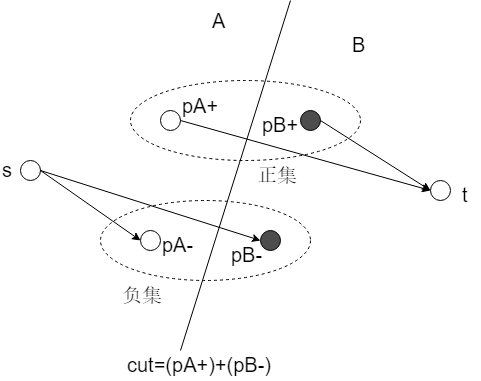
\includegraphics[scale=0.6]{image/networkflow11.png}
  \caption{项目选择问题一般情形}\label{fig11}
\end{figure}

\begin{itemize}
\item 解的可行性:该模型s的所有出边容量为有限值,最坏的情况就是所有负价值点都被选入,此时最小割为s所有出边,因此最小割是包含不到无穷大的边的,此解法也就是可行的。
\item 解为最优解:如\autoref{fig11}为此模型获得的一般割情形。
\end{itemize}
从\autoref{fig11}可求此结果的价值:
\begin{equation}
v = (p_{B+}) - (p_{B-}) = (p_+) - (p_{A+}) - (p_{B-}) = (p_+) - [(p_{A+}) + (p_{B-})] = (p_+) - cut\\
\end{equation}
所以所得价值为一常数减去割,要求\(maxv\),则割要为\(mincut\),即\(maxv = (p_+) -mincut\)

\chapter{分治算法之平面最近点对问题}

\begin{introduction}
\item 平面最近点对问题定义
\item 分治算法设计
\item 分治算法时间复杂度分析
\item 伪代码
\end{introduction}

\section{平面最近点对问题定义}
给定二维平面上的$n(n \ge 2)$个不同的点$p$组成点集$P = \{p_i \big| 1\le i \le n\}$,
设计算法寻找欧式距离最近的点对$(A,B)$。
\begin{figure}[htb]
    \centering
    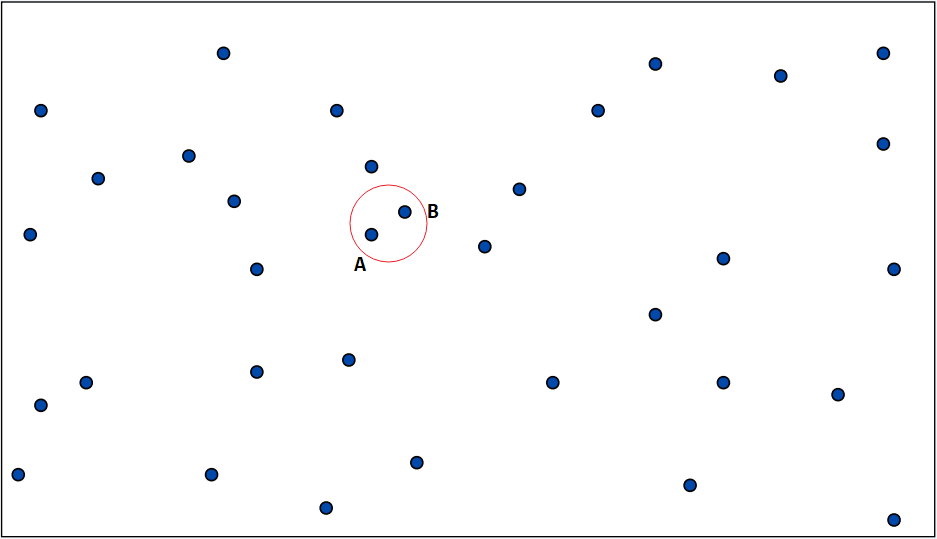
\includegraphics[scale=0.5]{Ln9.image/NearestPointsDef.png}
    \caption{问题定义图例}\label{fig1}
\end{figure}

如上图\autoref{fig1}中点对$(A,B)$即为问题的答案。

\section{分治算法设计}
对于这样一个问题,我们很直接地可以使用BF (Brute Force)算法进行暴力求解,
即二重循环计算所有点之间的距离,从而获得最小距离,显然该算法的时间复杂度为
$O(n^2)$。那么有没有更快的算法呢?本章我们使用经典的算法思想——分治,
设计一个$O(n\log n)$的算法。

\subsection{分治问题}
遵循分治思想,我们首先要考虑如何分治问题使得问题规模约减。

我们使用X坐标作为第一关键字、Y坐标作为第二关键字,对点集$P$进行排序,
并以点$p_{\lfloor\frac{n}{2}\rfloor}$作为分治点,获得如下两个点集:
\begin{equation*}
    P_1 = \{p_i\ \big|\ 1 \le i \le \lfloor\frac{n}{2}\rfloor \}
\end{equation*}
\begin{equation*}
    P_2 = \{p_i\ \big|\ \lfloor\frac{n}{2}\rfloor < i \le n\}
\end{equation*}
这样就将当前问题约减为两个规模为$\frac{n}{2}$的子问题
分治过程如\autoref{fig2}中所示。

\begin{figure}[htb]
    \centering
    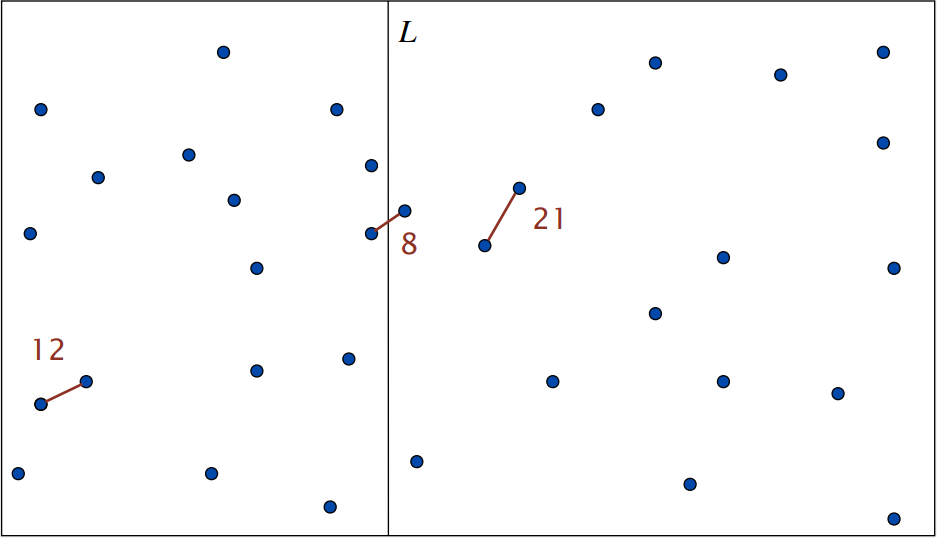
\includegraphics[scale=0.5]{Ln9.image/NearestPointsDivide.png}
    \caption{分治过程图例}\label{fig2}
\end{figure}

如此递归下去,我们可以求得两个点集相对应的最近点对距离$\delta_1, \delta_2$,取其中较小值
记为$\delta = \min \{ \delta_1 , \delta_2 \}$。

当分治到点集大小为2个或3个时,可以在常数时间内计算出子问题的解。

\subsection{合并结果}

接着,我们需要考虑如何合并子问题的解。

上述的$\delta$一定是正确的合并结果嘛?显然不是,我们并没有考虑,一端在$P_1$,
一端在$P_2$的线段。因此,在合并阶段,我们要将这种情况考虑在内。

这里,我们将所有横坐标与分治点$p_{\lfloor\frac{n}{2}\rfloor}$的横坐标
$x_{\lfloor\frac{n}{2}\rfloor}$差值小于$\delta$的点组成集合$B$,即
\begin{equation*}
    B = \{p_i\ \big|\ 
        \left|x_i - x_{\lfloor\frac{n}{2}\rfloor}\right| \le \delta ,\
        1 \le i \le n\}
\end{equation*}   
因为只有$B$集合中的点之间的距离才有可能小于$\delta$。
$B$集合如下图\autoref{fig3}中阴影部分所示:
\begin{figure}[htb]
    \centering
    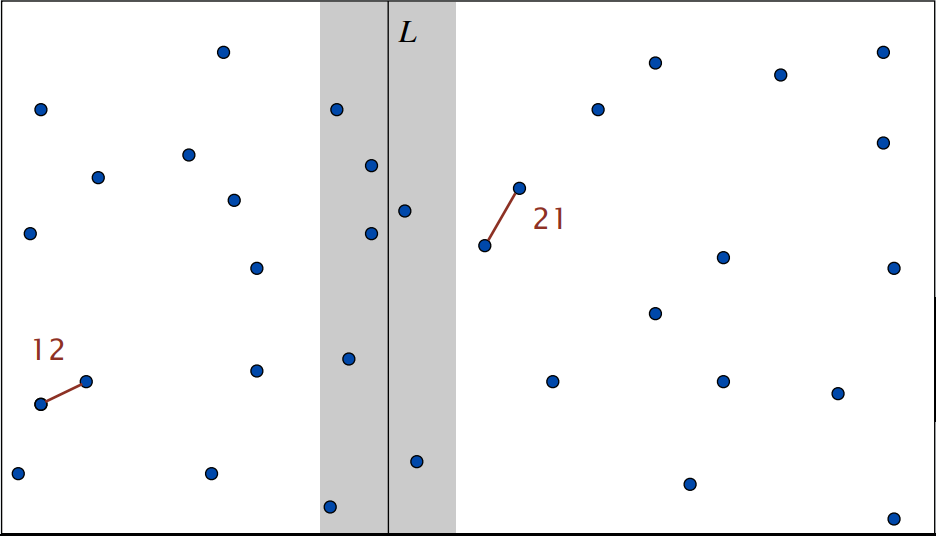
\includegraphics[scale=0.5]{Ln9.image/NearestPointsMerge.png}
    \caption{合并过程图例}\label{fig3}
\end{figure}

进一步,我们的目标是检验在$B$集合中是否存在距离比$\delta$更近的点对,以此更新当前问题的解
。因此,对于每个$p_i = (x_i, y_i) \in B$遍历所有在其之下竖直距离不超过$\delta$的点,
即遍历集合
\begin{equation*}
    C(p_i) = \{ p_j\ \big|\ y_i - \delta \le y_j \le y_i, p_j \in B \}
\end{equation*}
为了方便遍历,我们可能会想到对$B$集合中的点,以Y坐标为第一关键字,X坐标为第二关键字,进行排序。
但是如此一来,每一次合并的时间复杂度为$O(n \log n)$,徒增时间消耗,因此我们采取合并策略,即
按照Y坐标为关键字,进行$P_1, P_2$的归并来直接获得排序后的集合$B$,这样只需要$O(n)$的时间。

考虑到$C(p_i)$会因为归并操作而维持在$O(n)$数量级,其实不然,该集合的大小不会超过7。下面给出
证明。

根据定义,$C(p_i)$中的点的纵坐标均处于$(y_i - \delta, y_i]$范围内,且其中的所有点
的横坐标均处于$\left( x_m - \delta, x_m + \delta \right)$范围内。
这样便构成了一个$2\delta\times\delta$的矩形。如下图\autoref{fig4}所示
\begin{figure}[htb]
    \centering
    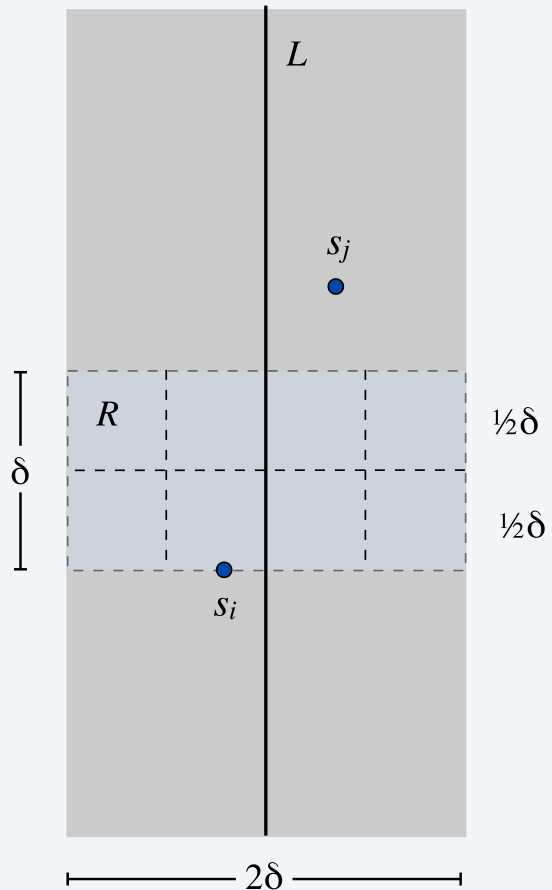
\includegraphics[scale=0.5]{Ln9.image/NearestPointsCpi.png}
    \caption{$C(p_i)$}\label{fig4}
\end{figure}。

接着,我们将这个矩形分拆成左右两个$\delta \times \delta$的正方形,左侧正方形的点集为
$C(p_i)\cap P_1$,右侧正方形的点集为$C(p_i)\cap P_2$,从上述的分治过程可知,这两个点集
内的点之间的距离一定不小于$\delta$。

进一步,我们将$\delta \times \delta$正方形,分拆成四个$\frac{\delta}{2}\times\frac{\delta}{2}$
小正方形,因为这个小正方形的对角线为$\frac{\delta}{\sqrt{2}} < \delta$,所以小正方形中最多
只有一个点,而总共有8个小正方形,最多有8个点,除去$p_i$,则最多只有7个点。

至此,我们完成了父问题的分治与子问题的合并。

\section{分治算法的时间复杂度分析}
首先,第一次排序可以使用时间复杂度为$O(n\log n)$的排序算法,如快速排序或者归并排序。

接着,我们考虑分治过程,即通过分治,我们将规模为$n$的父问题,分为两个规模为$\frac{n}{2}$的子问题。

最后,归并过程中,根据采用的合并策略以及上述对更新操作的证明,我们需要$O(n)$级别的时间完成。

综上,给出递推式如下:

\[
    T(n) = \begin{cases}
        O(1) & 2 \le n \le 3 \\ 
        2T(\frac{n}{2}) + O(n) & n > 3
    \end{cases} 
\]

推导如下:
\begin{align*}
        T(n) &= 2T(\frac{n}{2}) + O(n)\\
             &= 2^2T(\frac{n}{2^2}) + 2O(\frac{n}{2}) + O(n)\\
             &= 2^2T(\frac{n}{2^2}) + 2O(n)\\
             &\vdots \\
             &= 2^k T(\frac{n}{2^k}) + kO(n)\ \ (n = 2 ^ k)\\
             &= O(n) + O(n\log n) \\ 
             &= O(n\log n)
\end{align*}

\section{伪代码}
\begin{algorithm}
    \DontPrintSemicolon{}
    \KwData{
        Point List $P = \{p_i\ \big|\ 1 \le i\le n, p_i = (x_i, y_i)\}$\;
        $P$ should be sorted by x-coordinate in descending order.
    }
    \KwResult{the minimum distance $\delta$}
\Begin{
    \If{$\left| P \right| <= 3$}{ 
        Return the minimum Euclidean-Distance between each pair of points.
    }
    $m \leftarrow \lfloor \frac{n}{2} \rfloor$\;
    $\delta_1 \leftarrow \text{Nearest-Pair}(P[1,\ \ldots,\ m])$\;
    $\delta_2 \leftarrow \text{Nearest-Pair}(P[m + 1,\ \ldots ,\ n])$\;
    $\delta \leftarrow \min \{ \delta_1,\ \delta_2 \}$\;
    $B \leftarrow \text{MergeByY}(P_1,\ P_2)$\;
    \ForEach{$p_i \in B$}{
        \ForEach{$p_j \in C(p_i)$} {
            $\delta \leftarrow \min \{\delta,\ \text{Euclidean-Distance}(p_i, p_j)\}$
        }
    }
    Return $\delta$
}
\caption{Nearest-Pair\label{NPP}}
\end{algorithm}
\chapter{分治法之大数乘法}
\begin{introduction}
    \item 问题背景
    \item 直接分治法
    \item 改进分治法
\end{introduction}

\section{问题描述}
给定两个大数$A$和$B$, 试计算
\begin{math}
    A \times B
\end{math}.
其中$A$和$B$分别表示为
\begin{math}
    A = a_n a_{n-1} a_{n-2} \ldots a_2 a_1
\end{math}
,
\begin{math}
    B = b_n b_{n-1} b_{n-2} \ldots b_2 b_1
\end{math}.
根据已学知识,给出如下引理。

\begin{lemma}{}{label_for_a+b}
    直接计算$A + B$,其复杂度为$O(n)$, 其中$n$为$A$和$B$的十进制位数。
\end{lemma}

直接计算$A \times B$时,我们将$A$与$B$的各位相乘,在将各中间结果相加,得到最终结果。
不难得出,这一过程需要进行$n$次基本乘法与$n+1$次加法。
根据引理\ref{lem:label_for_a+b},有:
\begin{theorem}{}{label_for_a*b}
    直接计算$A \times B$的时间复杂度为$O(n^2)$.
\end{theorem}

由定理\ref{thm:label_for_a*b}和引理\ref{lem:label_for_a+b}可知,如果我们直接相乘两个大数,其时间复杂度相比加法运算高出一个量级。
由于乘法在计算机中大量存在,我们希望找到更好的算法来降低乘法计算的时间复杂度,以提升计算机的性能。
分治法为我们提供了一条途径。
\section{直接分治法}
\subsection{算法描述}
这是一种简单的分治方法,将两个大数分为前后两部分,进行相乘。不失一般性,这里假设$n$为偶数。
将$A$与$B$分割为$A_2$, $A_1$, $B_2$, $B_1$,即:
\begin{displaymath}
    \begin{split}
        A_2 &= a_{n} a_{n-1} \ldots a_{\frac{n}{2} + 2} a_{\frac{n}{2} + 1}\\
        A_1 &= a_{\frac{n}{2}} a_{\frac{n}{2} - 1} \ldots a_2 a_1\\
        B_2 &= b_{n} b_{n-1} \ldots b_{\frac{n}{2} + 2} b_{\frac{n}{2} + 1}\\
        B_1 &= b_{\frac{n}{2}} b_{\frac{n}{2} - 1} \ldots b_2 b_1
    \end{split}
\end{displaymath}

则$A$可以写为$A = A_2 \times 2^{\frac{n}{2}} + A_1$.
$B$可以写为$B = B_2 \times 2^{\frac{n}{2}} + B_1$.
计算$A \times B$的问题在进行上述转换后表示为:
\begin{displaymath}
    \begin{split}
        A \times B
        & = (A_2 \times 2^{\frac{n}{2}} + A_1) \times (B_2 \times 2^{\frac{n}{2}} + B_1) \\
        & = A_2 B_2 \times 2^n + (A_2 B_1 + A_1 B_2) \times 2^{\frac{n}{2}} + A_1 B_1
    \end{split}
\end{displaymath}

此时将两个大数相乘的问题转化为4个乘法子问题和3个加法子问题。显然,分治策略还可以对子问题使用,继续减小问题的规模。

\subsection{伪代码}
\begin{algorithm}
    \DontPrintSemicolon{}
    \KwIn{Two large numbers $A$, $B$, which both have $n$ decimal digits}
    \KwResult{$A \times B$}
    \Begin{
        $n \leftarrow $ Number of Decimal Digits of $A$ and $B$\;
        \If{$n \neq 1$}{
            Divide $A$, $B$ into $A_2$, $A_1$, $B_2$ and $B_1$\;
            $C_3 \leftarrow DirectDAC(A_2, B_2)$\;
            $C_2 \leftarrow DirectDAC(A_2, B_1)$\;
            $C_1 \leftarrow DirectDAC(A_1, B_2)$\;
            $C_0 \leftarrow DirectDAC(A_1, B_1)$\;
            \KwRet{$C_3 \ll n + (C_2 + C_1) \ll (n - 1) + C_0$}\;
        }
        \Else{
            \KwRet{$A \times B$}
        }
    }
    \caption{DirectDAC\label{label_for_pseudo_DirectDAC}}
\end{algorithm}

\subsection{复杂度分析}
由上述的算法描述可知,算法的主要开销来自于每次分支带来的4个乘法子问题和3个加法子问题,由于移位可在机器中由一个简单的指令完成,我们忽略这个操作的时间。\\
假设$T(n)$表示两个$n$位大数相乘所需的时间开销,则在直接分治法中:
\begin{displaymath}
    \begin{split}
        T(n)
        &= 4T(\frac{n}{2}) + 3n \\
        &= 4T(\frac{n}{2}) + O(n)
    \end{split}
\end{displaymath}

根据主方法,$\log_2 4  = 2> 1$, 推出如下定理:
\begin{theorem}{}{label_for_DirectDAC_complexity}
    用直接分治法计算$A \times B$的时间复杂度为$O(n^2)$.
\end{theorem}

根据定理\ref{thm:label_for_DirectDAC_complexity},直接分治法的性能是令人失望的,因为其并不能提供时间上优于直接相乘的性能。
但分治策略提示我们,这个算法的性能与乘法子问题的数目强相关。我们如果能够用一些其他的开销换取更少的乘法子问题数目,也许能得到更好的算法。


\newpage
\section{改进分治法}
\subsection{改进思路}
在直接分治法中,通过对大数进行分割,我们有:
\begin{displaymath}
    A \times B = A_2 B_2 \times 2^n + (A_2 B_1 + A_1 B_2) \times 2^{\frac{n}{2}} + A_1 B_1
\end{displaymath}

这个过程中,引入了4次乘法运算;在上一节中提到,分治策略和主定理提示我们尽可能减少乘法的次数。
但换取更低的乘法子问题数,需要其他的开销。
一种想法是,由于加法的复杂度为$O(n)$,我们也许可以用略多的加法子问题,来减少乘法子问题数。
基于此想法,我们对直接分治法作出一些改进。首先将直接分治法中的计算式修改为:
\begin{displaymath}
    \begin{split}
        A \times B
        &= A_2 B_2 \times 2^n + (A_2 B_1 + A_1 B_2) \times 2^{\frac{n}{2}} + A_1 B_1\\
        &= A_2 B_2 \times 2^n + ((A_2 + A_1)\times(B_2 + B_1) - A_2 B_2 - (A_1 B_1)) \times 2^{\frac{n}{2}} + A_1 B_1
    \end{split}
\end{displaymath}

观察上式,我们只需要做3次乘法,即计算$A_2 B_2$, $A_1 B_1$, $(A_2 + A_1)\times(B_2 + B_1)$, 以及4次加法,2次减法。
考虑到加法和减法本质上等同,我们成功地将这一问题转化为了3个乘法子问题和6个加法子问题。相比于直接分治法,我们降低了乘法的数量。

下面给出该算法的伪代码及复杂度分析。
\subsection{伪代码}
\begin{algorithm}
    \DontPrintSemicolon{}
    \KwIn{Two large numbers $A$, $B$, which both have $n$ decimal digits}
    \KwResult{$A \times B$}
    \Begin{
        $n \leftarrow $ Number of Decimal Digits of $A$ and $B$\;
        \If{$n \neq 1$}{
            Divide $A$, $B$ into $A_2$, $A_1$, $B_2$ and $B_1$\;
            $C_2 \leftarrow DirectDAC(A_2, B_2)$\;
            $C_1 \leftarrow DirectDAC(A_1, B_1)$\;
            $C_0 \leftarrow DirectDAC(A_2 + A_1, B_2 + B_1)$\;
            \KwRet{$C_2 \ll n + (C_0 - C_2 - C_1) \ll (n - 1) + C_1$}\;
        }
        \Else{
            \KwRet{$A \times B$}
        }
    }
    \caption{ModifiedDAC\label{label_for_pseudo_ModifiedDAC}}
\end{algorithm}

\subsection{复杂度分析}
同上节的复杂度分析,我们此处也忽略移位操作带来的开销。改进分治法中,我们将问题分解为3个乘法子问题与6个加法子问题。
因此有:
\begin{displaymath}
    \begin{split}
        T(n)
        &= 3T(\frac{n}{2}) + 6n\\
        &= 3T(\frac{n}{2}) + O(n)
    \end{split}
\end{displaymath}

根据主方法,$\log_2 3 > 1$. 推出如下定理:
\begin{theorem}{}{label_for_ModifiedDAC_complexity}
    用改进分治法计算$A \times B$的时间复杂度为$O(n^{\log_2 3}) \approx O(n^{1.585})$.
\end{theorem}

\bibliography{ref.bib}
\end{document}
